\section{Data visualisation}

\subsection{Definition}
A number of definitions have been proposed to explain what data visualisation means. According to Friendly \cite{Friendly2009} the term came together with the birth of statistical thinking as a way to illustrate mathematical language, their trends, tendencies and distributions through the use of diagrams and graphics. Few \cite{StephenFew2013} describes it as a graphical display of abstract information for the purpose of sense-making and communication. 
However, this definition does not exclude representations that are not algorithmically drawn. The definition offered by Iliinsky and Steele \cite{Iliinsky2011} is more specific: 
\begin{displayquote}
Any visual representation of data that is:
	\begin{itemize}
	\item algorithmically drawn (may have custom touches but is largely rendered with the help of computerized methods);
	\item easy to regenerate with different data (the same form may be repurposed to represent different datasets with similar dimensions or characteristics);
	\item often aesthetically barren (data is not decorated); and
	\item relatively data-rich (large volumes of data are welcome and viable, in contrast to infographics).
    \end{itemize}
\end{displayquote}
\iffalse
\begin{figure}[h]
  \centering
  \begin{adjustbox}{width=.8\textwidth,center=\textwidth}
  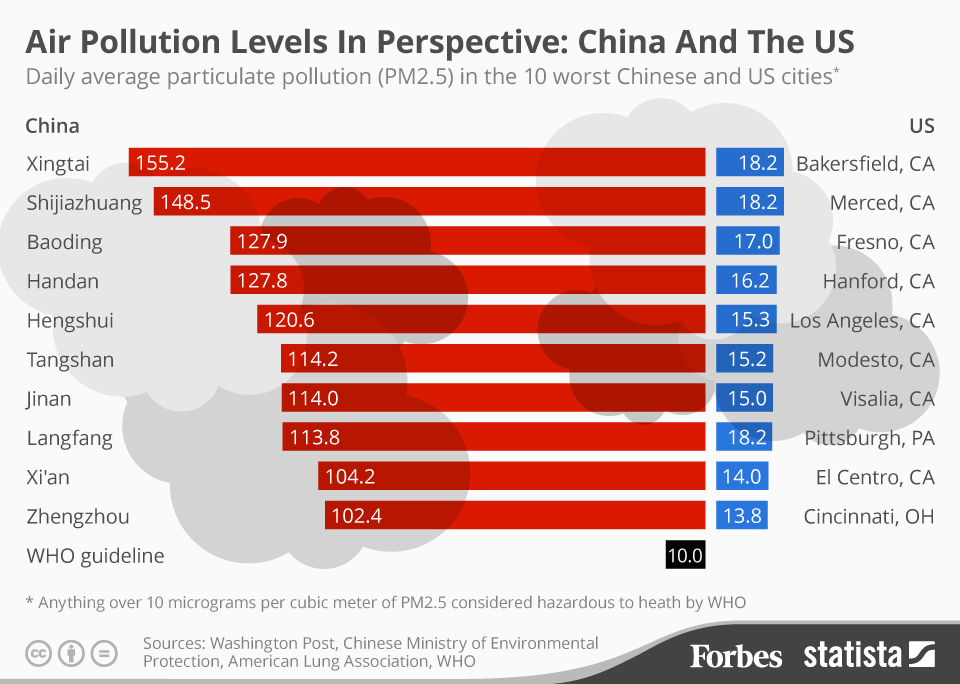
\includegraphics[scale=1]{images/air_pollution_infographic.jpg}
  \end{adjustbox}
  \caption[Air pollution infographic]{Air pollution infographic \cite{NiallMcCarthy}}
  \label{fig:air_pollution_infographic}
\end{figure}
\fi
A visualisation helps in the understanding of data  by taking advantage of the human visual system to process a large amount of information quickly, thus allowing the human brain to identify patterns, links and relationships between the represented objects. Daniel et al. \cite{KeimDaniel2010}, also states that visualising enables people to: 
\begin{displayquote}
	\begin{itemize}
\item  Synthesise information and derive insight from massive, dynamic, ambiguous, and often conflicting data.
\item Detect the expected and discover the unexpected.
\item Provide timely, defensible, and understandable assessments.
\item Communicate these assessment effectively for action.
	\end{itemize}
\end{displayquote}

Data visualisation is essential when the available data is vast and dynamic, and when raw data does not make sense on its own. Therefore, data must be encoded using technological and design elements;  potentially making use of disciplines such as statics, data mining, human computer interaction and graphic design. 

\subsection{Designing Data Visualisations}
Figure \ref{fig:data_visualization_process} depicts the visual analysis process according to Daniel et al. \cite{KeimDaniel2010}. In the first stage,  data should be collected, usually from many distinct data sources and standardised into one common format. This later enables us to choose between the creation of models, or visualisations. Models are an automated representation that requires data mining techniques whereas visualisations are manually constructed  representations that can be created through simple mapping from data to the visual context. Both representations are linked together to enable validation and refinement through iteration. The final stage is arguably the most important as it is concerned with the knowledge gained from the representation and aims to respond the questions posed from the study in the first place.
\begin{figure}[!htb]
\begin{adjustbox}{width=1\textwidth,center=\textwidth}
  \centering

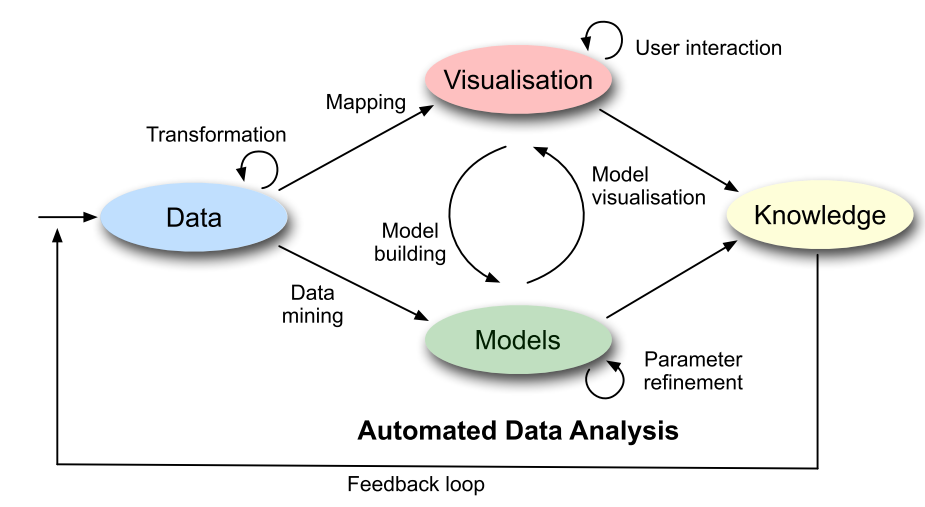
\includegraphics[scale=1]{images/data_visualization_process.png}
\end{adjustbox}
  \caption[The data visualisation process]{The data visualisation process \cite{KeimDaniel2010}. }
  \label{fig:data_visualization_process}
\end{figure}

According to Ben Fry \cite{Cleveland1993}, one specific approach for data visualisations is illustrated in Figure \ref{fig:data_visualization_stages}, which establishes a common series of steps that can be followed for this purpose:

\begin{displayquote}
	\begin{itemize}
\item Acquire: Obtain the data, whether from a file on a disk or a source over a network. 
\item Parse: Provide some structure for the data’s meaning, and order it into categories. 
\item Filter: Remove all but the data of interest. 
\item Mine: Apply methods from statistics or data mining as a way to discern patterns or place the data in mathematical context.
\item Represent: Choose a basic visual model, such as a bar graph, list, or tree. 
\item Refine: Improve the basic representation to make it clearer and more visually engaging. 
\item Interact: Add methods for manipulating the data or controlling what features are visible.
\end{itemize}
\end{displayquote}

\begin{figure}[!htb]
\begin{adjustbox}{width=1\textwidth,center=\textwidth}
  \centering
  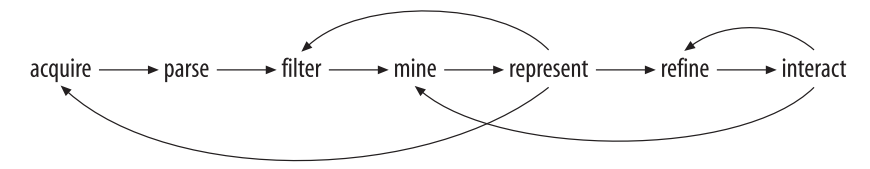
\includegraphics[scale=1]{images/visualization_stages.png}
\end{adjustbox}
  \caption[Visualisation stages]{Visualisation stages  \cite{Cleveland1993}. }
  \label{fig:data_visualization_stages}
\end{figure}
From this perspective, it is possible to establish that all visualisations require an elemental process guided by the designer to enable the recognition of patterns within the data. Also that the design process is an iterative task where the designer may go back to redefine any stage of the process until the desired result is achieved. 

\subsection{Data Visualisations for Decision Support}
Caroll, Anderson, Olson et al. established in their analysis of human-computer interaction that
\quotes{a decision-making process usually includes the acquisition of related information, the construction of a mental representation of the problem and solutions, and the identification of an optimal solution} \cite{carroll1987mental} as cited in \cite{Zhu2008}, decision making involves acquiring domain-specific information about a particular question which is the intended output of a data visualisation. Therefore, it is important to understand the effects of data visualisations in decision support.

The decision-making process takes into account the decision maker's skill, the task of making a decision and the problem space. In our specific context, the decision maker should be able to understand the data in its represented space (visualisation), evaluate the problem (avoid air pollution) and execute a decision task (leave the polluted space). \quotes{A well-designed visualisation takes features of the decision task and the characteristics of the decision makers into consideration} \cite{Zhu2008}. Thus, visualisations should be created in the specific context of the decision makers; discovering beforehand the knowledge they should have, the problems they are likely to face, and the potential decisions they should be able to make. 
